\label{sec:theory-higgs}
\subsection{The Broken Symmetry}

Quarks, charged leptons and weak interaction gauge bosons have mass. From the Lagrangian shown in last section, at this point, it does not explicitly provide mass to these particles. The mechanism through which these particles acquire mass is called spontaneous symmetry breaking.

Recall that the Higgs potential is of the from $V(\phi)=(\frac{1}{2}\mu^2\phi^{\dagger}\phi+\lambda(\phi^{\dagger}\phi )^2)$. Let us denote the two components of the Higgs comples doublet as $\phi^+ = \frac{\phi_1+i\phi_2}{\sqrt{2}}$ and $\phi^0 = \frac{\phi_3+i\phi_4}{\sqrt{2}}$. If the term $\mu^2<0$, then the potential follow a Mexican hat shape in the 2-dimensional space as shown in Fig.\ref{fig:theory-mexican} and has a minimum at $\phi^{\dagger}\phi = \frac{-\mu^2}{2\lambda} = \frac{\nu^2}{2}$, i.e. the Higgs field acquires a vacuum expectation value. Let us now expand the theory among the direction where $\phi_0 = \frac{1}{\sqrt{2}}\begin{psmallmatrix*}[r]0\\ \nu+H \end{psmallmatrix*}$, i.e. $\phi_3=\nu+H$ and  $\phi_1=\phi_2=\phi_4 = 0$. Once we have chosen a specific direction, the $SU(2)\times U(1)$ symmetry is broken.


\begin{figure}[htpb!]
\begin{center}
  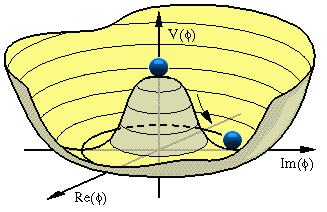
\includegraphics[width=0.45\linewidth]{figures/theory/MexicanHat.png}
\caption{Mexican Hat Potential}
\label{fig:theory-mexican}
\end{center}
\end{figure}


Now, recall from Eq.\ref{eq:l-su21}, since $D_{\mu}$ takes the form in Eq.\ref{eq:SU2U1D}, the covariate derivative of $\phi$ contains a term as shown in Eq.\ref{eq:SU2U1cov}, where three degree of freedoms of the original $SU2$ and $U1$ gauge bosons now have mess terms and transform to physical massive $W^{\pm}$ and $Z$ bosons, and one degree of freedom remains massless as the physical photon $\gamma$. 

\begin{equation}
 D_{\mu}  = \partial_{\mu}-ig_1\frac{Y}{2}B_{\mu} - ig_2\frac{\sigma}{2}W_{\mu}
  \label{eq:SU2U1D}
\end{equation}


\begin{equation}
  \begin{split}
   &\phi^{\dagger}(ig_1\frac{Y}{2}B_{\mu}+ig_2\frac{\sigma}{2}W_{\mu})^{\dagger} (ig_1\frac{Y}{2}B_{\mu}+ig_2\frac{\sigma}{2}W_{\mu}) \phi  \\
   =& (\frac{1}{2}\nu g_2)^2 W_{\mu}^+W^{-\mu} + \frac{1}{2}(\frac{1}{2}\nu \sqrt{g_1^2+g_2^2})^2 Z_{\mu}Z^{\mu} + \text{H field terms, where}\\
   &W^{\pm} = \frac{1}{\sqrt{2}}(W^1\mp iW^2) \text{, } Z = -\sin{\theta_W}B+\cos{\theta_W}W^3 \text{ and } \cos{\theta_W} = \frac{g_2}{\sqrt{g^2_1+g^2_2}}
  \end{split}
  \label{eq:SU2U1cov}
\end{equation}


Similarly, the Yukawa couplings in Eq.\ref{eq:l-su21} after symmetry breaking gives mass to the fermions. The expanded terms for electron, for example, is $\mathcal{L} = m_e\bar{e} e + \frac{m_{e}}{\nu}\bar{e}e H$. Two aspects of lepton mass worth commenting. First, in Standard Model there are no right handed neutrinos, hence the neutrinos do not interact with the Higgs boson. Secondly the coupling of lepton fields with higgs has a strength which is proportional to the mass of the lepton. Hence the heavier the lepton fields are, the stronger the interaction is. For quarks, one more complication arises. The Yukawa coupling is not diagonal. Generations of quarks can mix through the CKM matrix.

Finally the Higgs boson gets its own mass through self-interaction term in the Higgs potential after symmetry breaking. The free parameters of the Standard Model have thus been all revealed to us. There are 9 mass parameters for the fermions and 4 parameters for the quark CMK matrix. Each gauge symmetry gets one free coupling parameter while the strong interaction has one more parameter called QCD vacuum angle. On the Higgs side, the vacuum expectation and Higgs mass are free parameters. In total, the theory has 19 free parameters. All parameters, with the Higgs mass measured by Run I ATLAS and CMS experiments measured to be roughly 125\GeV, have been revealed. 


\subsection{Higgs Phenomenology}

The Standard Model Lagrangian dictates the possible Higgs couplings. On the decay side, the Higgs branching ratio is shown in Fig. \ref{fig:theory-higgsbr}. At $M_H = 125\GeV$, the most probable decay mode of Higgs is \Hbb. Recall that the Higgs to fermion coupling strength is proportional to the fermion mass. Although the top quark is way heavier than the bottom quark, the Higgs is not heavy enough to produce on-shell top pairs. On the production side, the Higgs production cross sections of different modes are shown in Fig. \ref{fig:theory-higgsp}. The Feymann diagrams of the leading four production modes: (1) gluon fusion-ggF (2) vector boson-VBF fusion (3) associated production and (4) $t\bar{t} H$ production are shown in Fig. \ref{fig:theory-higgsfeymann}


\begin{figure}[htpb!]
\begin{center}
  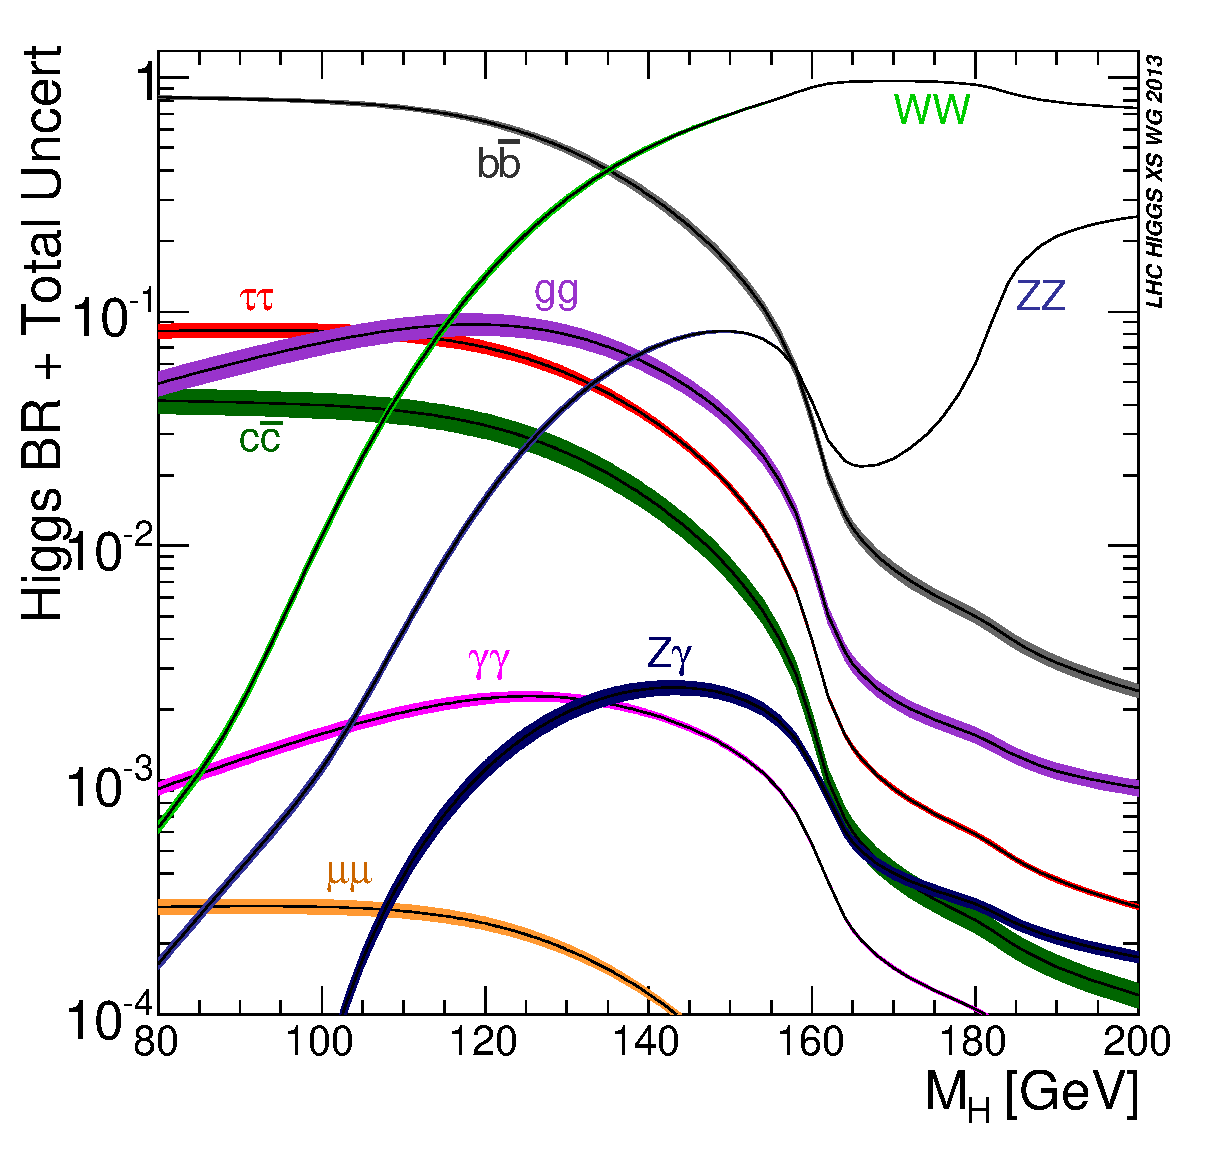
\includegraphics[width=0.45\linewidth]{figures/theory/Higgs_BR_LM.eps}
\caption{Higgs Branching Ratios as a function of hypothetical Higgs mass}
\label{fig:theory-higgsbr}
\end{center}
\end{figure}

\begin{figure}[htpb!]
\begin{center}
  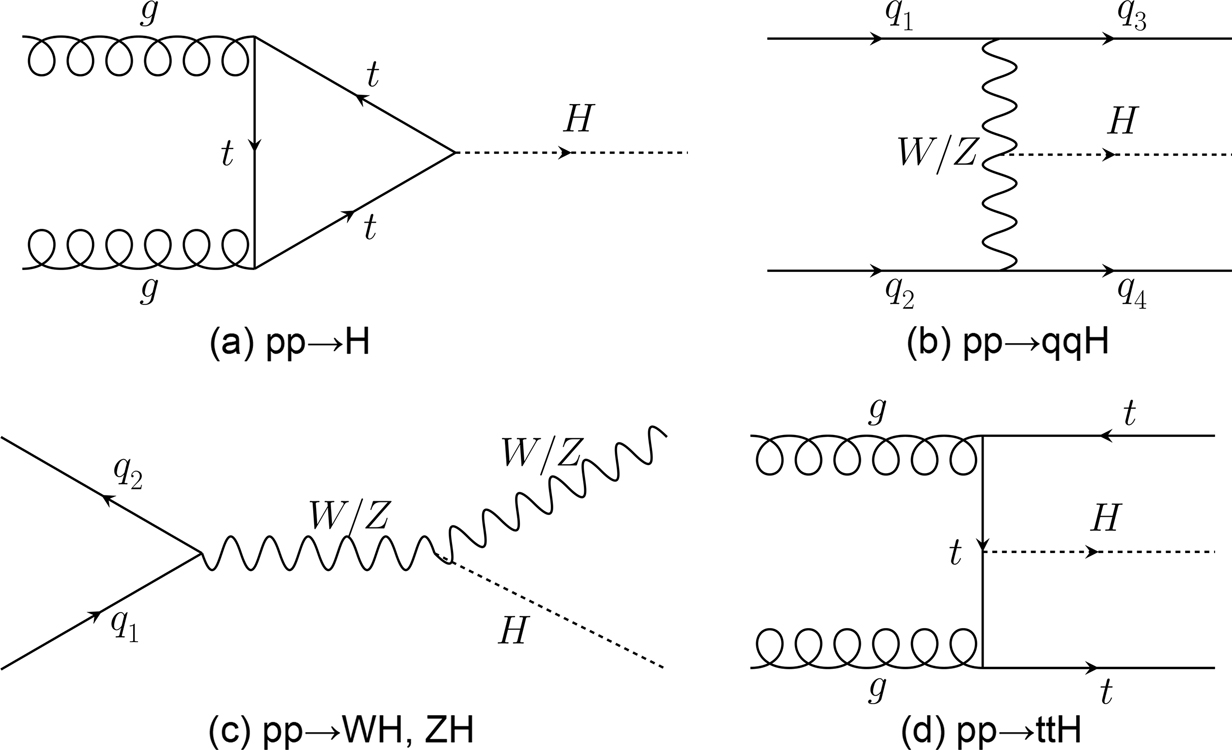
\includegraphics[width=0.45\linewidth]{figures/theory/ProductionFeymann}
\caption{Leading Higgs production Feymann Diagrams ranked in order of strength from (a) to (d)}
\label{fig:theory-higgsfeymann}
\end{center}
\end{figure}


To establish a discovery, particle physics community has agreed on that the observation of the signal significance roughly goes as $\frac{S}{\sqrt{B}}$ have to be greater than $5\sigma$. That is saying, in our measurements, the background-only model has less than $5.8\times 10^{-7}$ chance to fluctuate and generate the data we are seeing. Therefore, the sensitivity of Higgs search should not only consider the cross section of a specific channel which is the product of Higgs production cross section and branching ratio, but also take into account the irreducible backgrounds. The discovery of Higgs in 2012 was not made through gluon fusion with Higgs decaying to bottom quarks, which has the largest cross section, but through three channels \Hgammagamma, $h\rightarrow ZZ^{(*)}$ and $h\rightarrow WW^{(*)}\rightarrow l\nu l\nu$\cite{HIGG-2012-27,CMS-HIG-12-028}, as the Standard Model di-photon and di-boson processes are orders of magnitude weaker than fully hadronic final state QCD processes. The combination of Run I 7 and 8 \tev data also found evidence of the Higgs Yukawa coupling to $\tau$ with greater than $3\sigma$ significance through the combination of its $\tau_{\text{lep}}\tau_{\text{lep}},\tau_{\text{lep}}\tau_{\text{had}}$ and $\tau_{\text{had}}\tau_{\text{had}}$ decays \cite{HIGG-2013-32,CMS-HIG-13-004}. Meanwhile, the Run I searches of \Hbb decay were not conclusive. ATLAS and CMS searches measured signal significance to be 1.4 and 2.1 (2.6 and 2.1 expected)\cite{HIGG-2013-23,CMS-HIG-13-012}. The Higgs to quark Yukawa coupling still remains to be confirmed. 



\begin{figure}[htpb!]
\begin{center}
  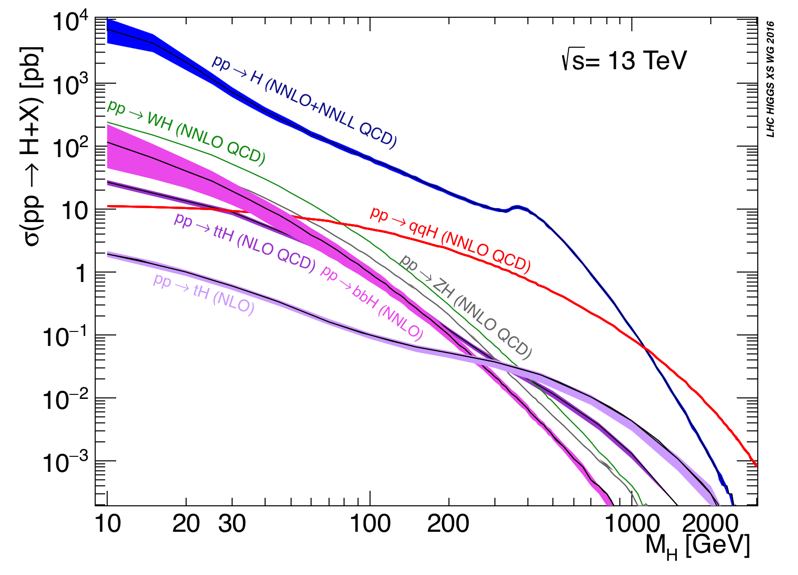
\includegraphics[width=0.6\linewidth]{figures/theory/HiggsCrossSection.png}
\caption{Higgs Production Cross Section at $\sqrt{s}= 13\tev$}
\label{fig:theory-higgsp}
\end{center}
\end{figure}
